\documentclass[conference]{IEEEtran}

\usepackage{cite}
\usepackage{amsmath,amssymb}
\usepackage{booktabs}
\usepackage{graphicx}
\usepackage{placeins}
\usepackage{float}
\usepackage{balance}
\usepackage{array}
\usepackage{url}
\usepackage[justification=centering,labelsep=period,font=footnotesize,skip=2pt]{caption}

\graphicspath{{generated/}}
\DeclareGraphicsExtensions{.pdf,.png}
\setlength{\textfloatsep}{5pt plus 2pt minus 2pt}
\setlength{\dbltextfloatsep}{5pt plus 2pt minus 2pt}
\setlength{\floatsep}{4pt plus 1pt minus 1pt}
\setlength{\abovecaptionskip}{3pt}
\setlength{\belowcaptionskip}{0pt}

\title{AERIS: Adaptive Environment-Aware Routing for IoT Sensors under Heterogeneous WSN Channels}

\author{
\IEEEauthorblockN{Anonymous Author(s)}
\IEEEauthorblockA{Submission for IEEE LCN 2026 (double-blind review)}
}

\begin{document}

\maketitle

\begin{abstract}
AERIS (\textit{Adaptive Environment-aware Routing for IoT Sensors}) is a fixed-rule hierarchical routing protocol designed for wireless sensor networks (WSNs) operating under heterogeneous channel conditions. The design integrates context-adaptive intra-cluster forwarding, Gateway-assisted cluster-head-to-base-station (CH-to-BS) uplinks, and a sparse Skeleton reserve backbone. Extensive evaluation in NS-3 against LEACH, PEGASIS, HEED, TEEN, and simplified collection-tree (CTP/RPL-MRHOF) baselines---spanning 50--1000 nodes across four environments---delineates a clear deployment boundary rather than universal superiority. While AERIS achieves rank-1 performance in 21 of 28 test cells against classical protocols, the inclusion of collection-style baselines localizes its competitive advantage to outdoor suburban settings. A 3360-run ablation study and a 400-replicate mechanism analysis attribute these gains primarily to Gateway-assisted uplinks, while identifying a fundamental engineering trade-off: accelerated first-node death (FND) in large-scale, harsh regimes. Consequently, AERIS serves as a reliability-first mechanism for specific harsh environments requiring auditable control, rather than a general-purpose replacement for mature collection-tree stacks.
\end{abstract}

\begin{IEEEkeywords}
wireless sensor networks, reliable routing, cross-platform evaluation, deployment boundary
\end{IEEEkeywords}

\section{INTRODUCTION}
Wireless sensor network (WSN) routing is traditionally evaluated through the lens of energy efficiency, yet in practical deployments, link stability often dictates the fundamental usability of a routing rule~\cite{akyildiz2002survey,rault2014energy,kandris2009power}. Classical protocols address this trade-off via distinct architectural priorities: LEACH focuses on clustered forwarding~\cite{heinzelman2000energy}, PEGASIS employs chain-based aggregation~\cite{lindsey2002pegasis}, HEED incorporates residual-energy-aware head election~\cite{younis2004heed}, and TEEN restricts reporting to event-triggered thresholds~\cite{manjeshwar2001teen}. In real-world scenarios, the problem is compounded because low-power WSN channels are inherently asymmetric, environment-sensitive, and prone to instability near connectivity thresholds~\cite{zuniga2004analyzing,zamalloa2007analysis,baccour2012radio}.

The practical engineering challenge is therefore not to identify a single dominant routing family, but to determine the specific regimes where a simple, auditable controller outperforms classical energy-first designs, and where more sophisticated collection-tree or RPL-style stacks remain the optimal choice. AERIS addresses this question through fixed-rule control rather than learned heuristics. Its architecture combines Context-Adaptive Switching (CAS) for intra-cluster mode selection, Gateway reinforcement for CH-to-BS uplinks, and a sparse Skeleton reserve backbone.

We make three primary contributions:
\begin{enumerate}
    \item We present AERIS as a fixed-rule routing design where online behavior is directly traceable to channel and topology inputs, ensuring deterministic control.
    \item We provide a comprehensive evaluation using a five-protocol NS-3 comparison and an expanded seven-protocol boundary sweep, including simplified CTP/RPL-MRHOF baselines and a collision-aware stress layer, while maintaining a clear separation between native ranking and stress-test evidence.
    \item Through extensive ablation and pooled trade-off statistics, we demonstrate that the reliability gains are primarily driven by Gateway support and are fundamentally paid for through earlier node death.
\end{enumerate}

\section{RELATED WORK}
Classical low-overhead WSN protocols continue to define the primary engineering operating points. LEACH and HEED mitigate long-range transmission costs via clustering, though their uplink quality remains highly sensitive to head placement and channel degradation~\cite{heinzelman2002application,younis2004heed}. PEGASIS distributes load through chain forwarding, but this robustness incurs the cost of increased latency and serialization~\cite{lindsey2002pegasis}. While TEEN suppresses redundant transmissions, its logic makes performance metrics sensitive to the specific definition of ``expected'' delivery~\cite{manjeshwar2001teen}. Collectively, these protocols represent the reliability-energy-latency trade-off that any contemporary design must confront.

Recent research has sought to improve reliability through machine learning, hybrid control, and context-aware adaptation~\cite{kumar2019machine,hu2024security,pushpa2025optimizing,tossa2025wireless,wang2024energy,khedr2025advancing,almutairi2025secured}. AERIS aligns with the objective of context-awareness but deliberately maintains a simple runtime logic: it relies on fixed coefficients and explicit control paths without training-time dependencies. Alongside a broader trend toward complex AI-driven routing and sophisticated LLN management documented in recent surveys~\cite{almutairi2024survey,djennadi2025exploring,thakur2025ai}, emerging designs frequently explore reinforcement learning and federated DDQN strategies~\cite{ren2023mefi,okine2024multi,singh2025enhanced,bhukya2025hybrid}.

Collection-tree and RPL-style protocols remain critical because they address the parent-selection problem through structured control planes. CTP constructs trees based on path quality~\cite{gnawali2009collection}, while RPL and MRHOF standardize DAG construction for lossy networks~\cite{tsvetkov2011rpl,gnawali2012minimum}. Opportunistic variants like ORW and ORPL further exploit link diversity~\cite{landsiedel2012low,duquennoy2013let}. This paper does not seek to replace these mature families. Instead, it investigates where a simpler fixed-rule design provides a sufficient reliability gain and where the established collection-tree paradigm should remain the default choice.

\begin{figure*}[t]
\centering
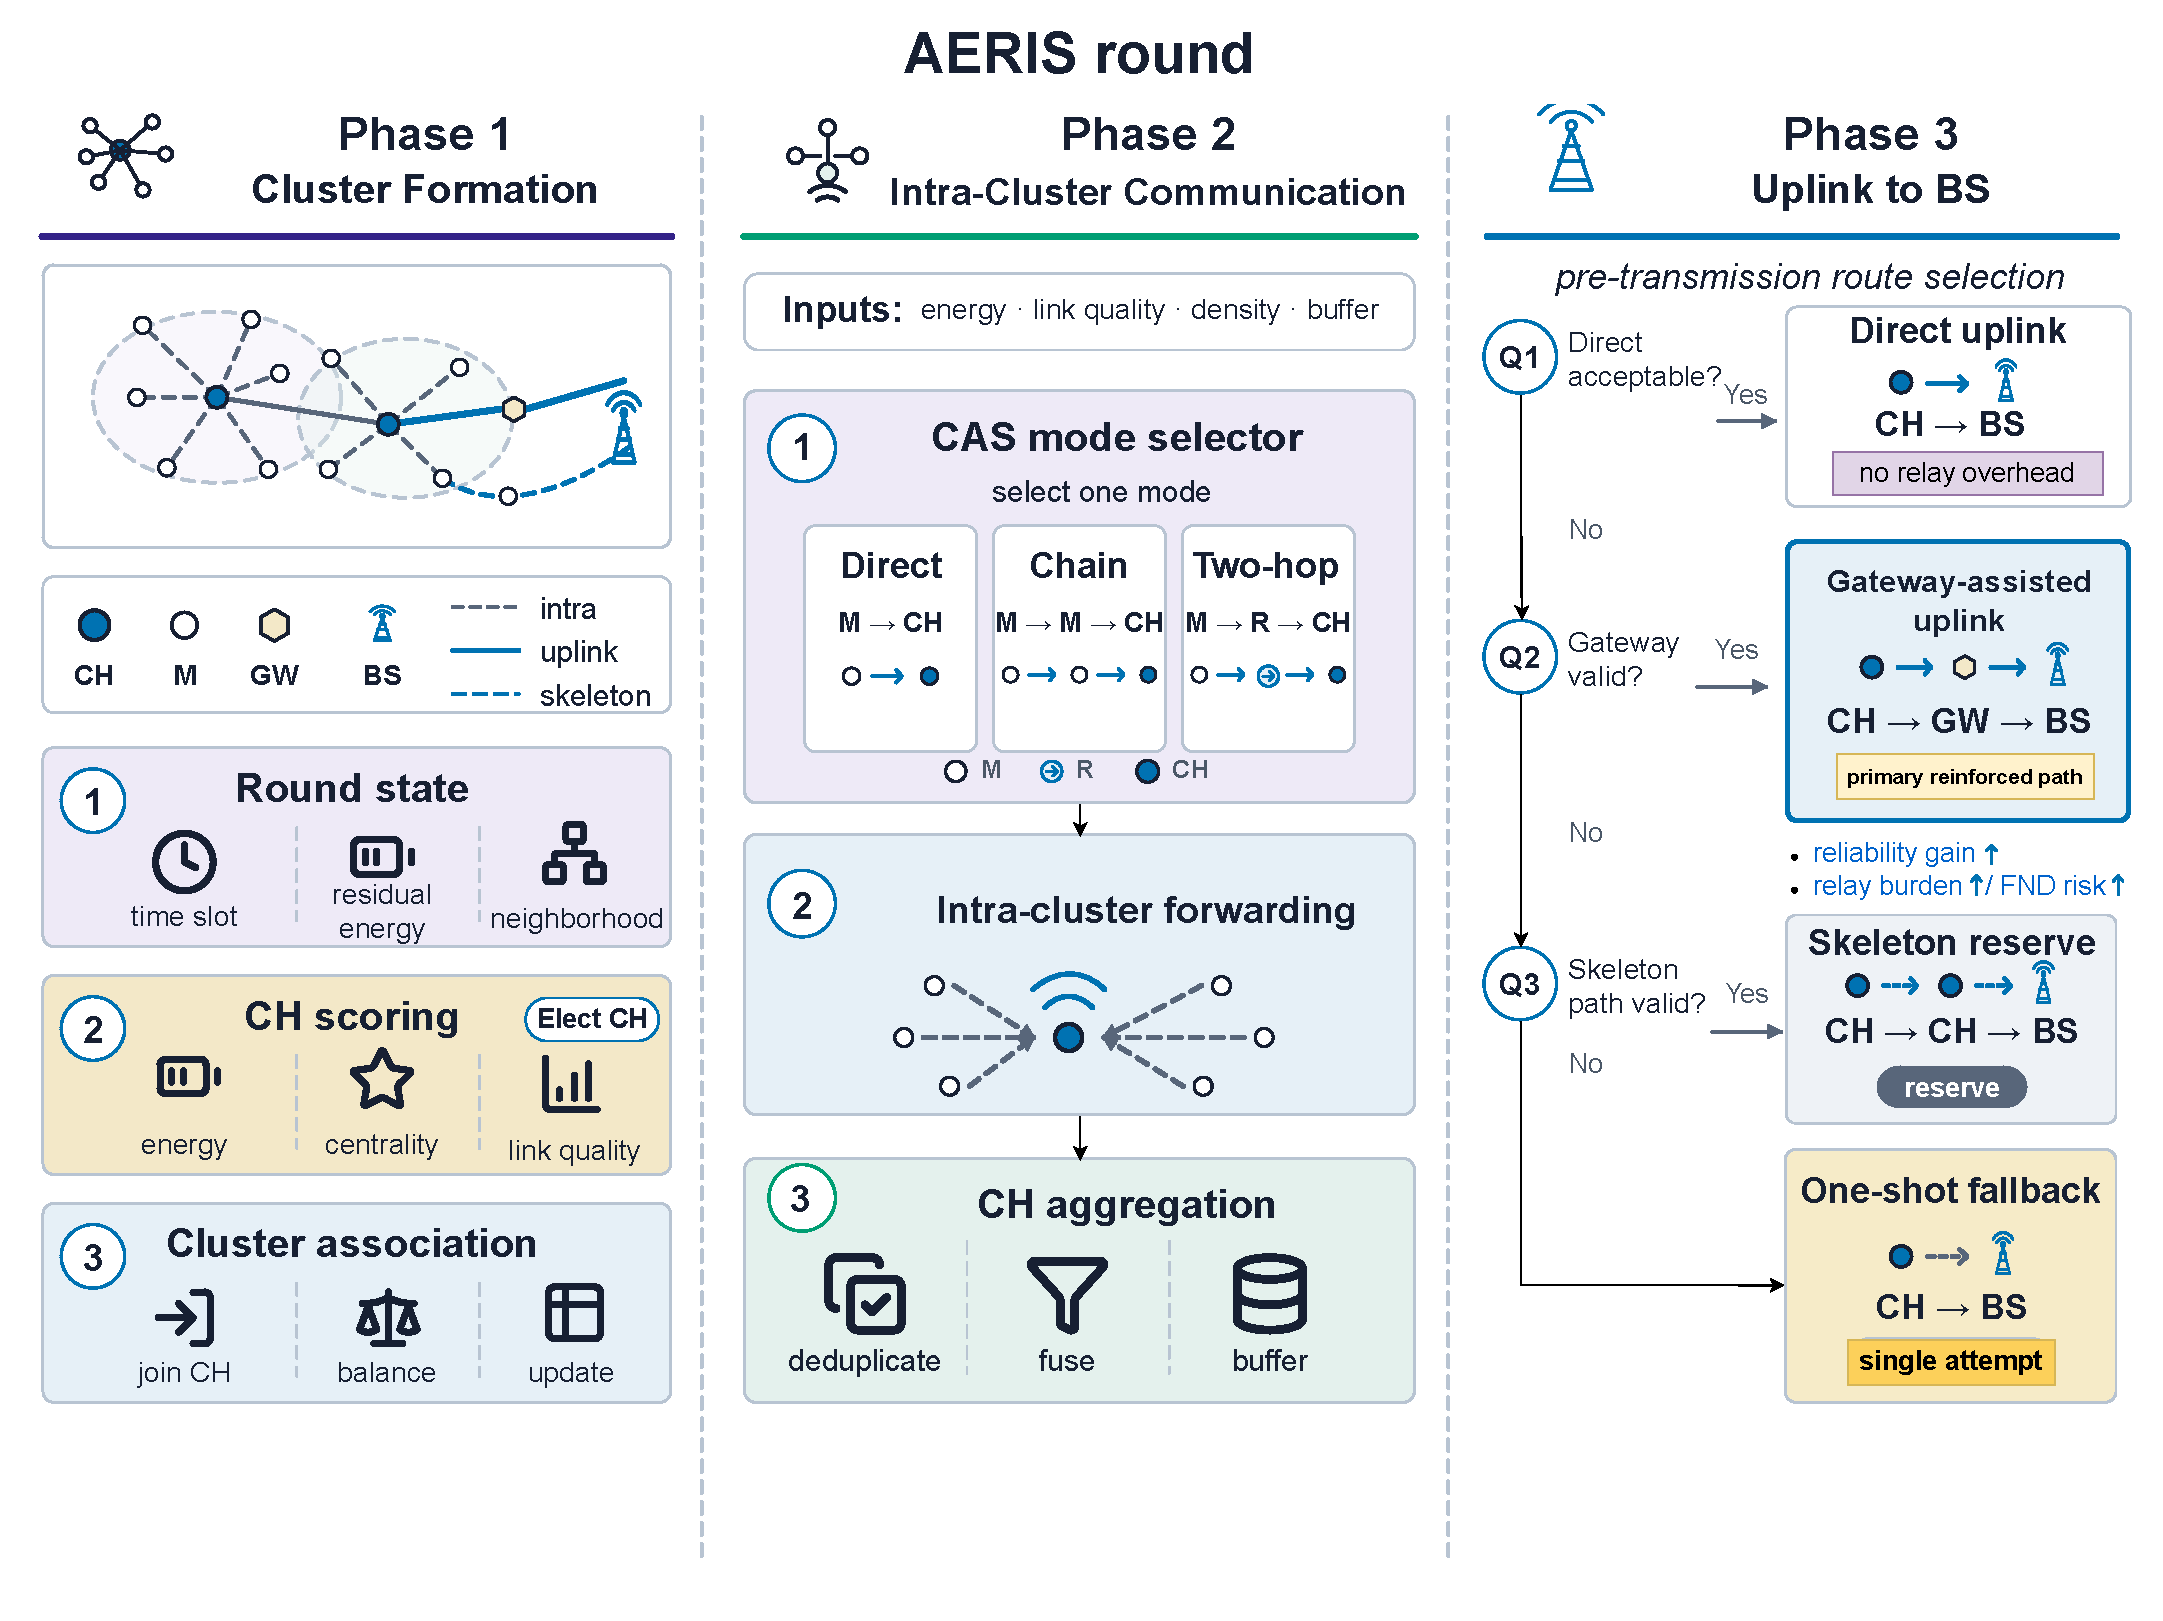
\includegraphics[width=0.92\textwidth]{AERIS_fig1_flow_chart.pdf}
\caption{AERIS round framework. The protocol first forms clusters and scores CH/Gateway candidates, then selects one CAS intra-cluster forwarding mode, and finally applies a first-hit uplink selector over direct, Gateway-assisted, Skeleton-reserve, and one-shot fallback paths.}
\label{fig:aeris_workflow}
\end{figure*}

\section{METHOD}
AERIS integrates CAS for intra-cluster mode selection, Gateway reinforcement for cluster-head-to-base-station uplinks, and a sparse Skeleton relay backbone as a reserve fallback. The design adds redundancy only where direct forwarding becomes fragile, while keeping the online control path deterministic and auditable. Figure~\ref{fig:aeris_workflow} summarizes the framework in the same order: cluster formation, intra-cluster communication, and pre-transmission uplink selection to the BS.

Gateway candidates are ranked by a fixed linear score,
\begin{equation}
\mathrm{Score}_i = \alpha \hat{E}_i + \beta \hat{C}_i + \gamma \hat{L}_i + \delta \hat{D}_i,
\end{equation}
where $\hat{E}_i$, $\hat{C}_i$, $\hat{L}_i$, and $\hat{D}_i$ denote normalized residual energy, centrality, link quality, and CH-to-BS distance. Centrality is a distance-aware neighborhood surrogate computed from local geometry; link quality is the current channel-estimated success probability for the candidate hop; and all scalar features are normalized to $[0,1]$ before scoring. Here $\hat{D}_i$ is the inverted normalized CH-to-BS distance score, so larger values indicate shorter distance.

CH candidates are scored separately by the fuzzy \texttt{cluster\_head\_chance} output of \texttt{FuzzyLogicSystem}, which combines residual energy, node centrality, node degree, distance-to-BS, and link quality; the top \texttt{cluster\_head\_ratio} fraction of alive nodes is then selected as CHs after a fairness penalty.

CAS uses another fixed linear rule over \{\text{direct, chain, two-hop}\}; the shared coefficients are fixed before all runs and are not tuned per environment:
\begin{equation}
m^{\star}=\arg\max_{m \in \{\mathrm{direct},\mathrm{chain},\mathrm{two\mbox{-}hop}\}} \left( a_m \hat{q} + b_m \hat{e} + c_m \hat{u} \right),
\end{equation}
where $\hat{q}$, $\hat{e}$, and $\hat{u}$ are normalized local channel quality, residual energy, and a per-CH utilization summary computed from local density and forward-buffer occupancy, and the coefficients $\{a_m,b_m,c_m\}$ are fixed for each candidate mode.

All core coefficients and thresholds are fixed before evaluation; the source defaults are $w_{\mathrm{dist}}=-0.7$, $w_{\mathrm{cent}}=0.3$, $w_{\mathrm{link}}=0.0$, and $w_{\mathrm{energy}}=0.0$ for Gateway, and \texttt{ema\_alpha}=0.2, \texttt{min\_confidence}=0.2, \texttt{lambda\_uncertainty}=0.0, and \texttt{uncertainty\_conf\_threshold}=0.4 for CAS, with the remaining mode weights and thresholds left unchanged from \texttt{CASConfig}; none are selected using environment-level test results. Skeleton forwarding is built as a sparse CH relay backbone after clustering and refreshed with the CH set; in this publication configuration it acts as a reserve fallback rather than an actively exercised mechanism.

The uplink logic is a first-hit selector rather than multipath routing. A cluster head checks direct uplink quality first, then tries Gateway support if a valid candidate exists, then Skeleton support if a reserve path is valid, and finally makes one last direct attempt. In the stress layer, this ``best-effort direct fallback'' is a single direct transmission attempt without protocol-level retransmission or transmit-power escalation.

In practice, CAS decides whether a sensor-to-CH transfer stays direct, switches to a short chain, or uses a two-hop relay; Gateway support then targets the more fragile CH-to-BS segment; Skeleton remains a reserve fallback if Gateway support is unavailable. AERIS is therefore evaluated as an engineering mechanism rather than claimed as a formal routing optimum: the same inputs trigger the same routing decisions, and the design is judged by how those decisions change delivery and cost in deployment.

\section{EXPERIMENTS}
\subsection{Experimental Setup}
The primary metric is packet delivery ratio over expected application-layer transmissions,
\begin{equation}
\mathrm{PDR}_{\mathrm{expected}}=\frac{N_{\mathrm{delivered}}}{N_{\mathrm{expected}}},
\end{equation}
where $N_{\mathrm{expected}}$ counts one packet per alive source node per round even if a protocol suppresses actual transmission. The denominator is kept fixed across protocols so that the reliability comparison is not confounded by protocol-specific reporting logic.

We use four complementary settings. A five-protocol NS-3 comparison evaluates AERIS against LEACH, PEGASIS, HEED, and TEEN across four environments and 100, 500, and 1000 nodes ($n=30$ per cell). An expanded NS-3 boundary sweep adds simplified CTP- and RPL-MRHOF-style collection baselines over 50--1000 nodes. In this standalone harness, CTP and RPL-MRHOF are simplified collection-style baselines rather than complete LLN stacks. Concretely, our CTP variant follows the link-cost forwarding rule of \cite{gnawali2009collection} but omits the 4-bit beacon-driven link estimator, dynamic beacon timer, and datapath validation; our RPL-MRHOF variant follows the path-cost parent selection of \cite{tsvetkov2011rpl,gnawali2012minimum} but omits trickle-driven DIO/DAO, full DODAG repair, and rank-based loop avoidance. These simplifications remove parts of the standards-compliant control plane and repair machinery, so the AERIS--baseline results should be read as a controlled collection-style boundary comparison; full Contiki-NG/TinyOS stacks may shift the boundary in either direction. Opportunistic variants such as ORW/ORPL \cite{landsiedel2012low,duquennoy2013let} and TSCH-based stacks \cite{duquennoy2015orchestra} are deferred to future work.

A 3360-run NS-3 ablation compares full AERIS with no-Gateway, no-CAS, and no-CH-score variants. A collision-aware Python stress layer adds explicit collision and relay contention; LEACH, HEED, and TEEN are minimally relay-enabled there for multi-hop comparability. The fixed 100-node block reports PDR, total energy, lifetime, first-node death, and hop count, while a 400-replicate-per-cell mechanism matrix explains which AERIS mechanisms actually fire.

For the NS-3 sweeps, nodes are uniformly placed in a 200 m $\times$ 200 m field with the sink at the top-center boundary; runs use 300 rounds, 512-byte packets, 2.0 J initial energy, 10 dBm transmit power, and seeds 42001--42030. The channel combines log-distance loss, shadowing, fading, receiver sensitivity, and packet-error probability. The path-loss/shadowing pairs are office (2.0, 4.5 dB), factory (2.7, 8.5 dB), suburban (2.8, 7.5 dB), and urban (3.4, 12.0 dB). The harness operates above an idealized contention-free MAC abstraction rather than the full IEEE 802.15.4 stack \cite{compatibility2023ieee}; the collision-aware Python stress layer adds explicit collision and relay contention on top of this abstraction.

The five-protocol NS-3 comparison anchors the classical-baseline ranking; the seven-protocol sweep maps the boundary against simplified collection-style baselines; the ablation attributes the gain; and the collision-aware stress layer provides stress evidence rather than a second canonical ranking. Lifetime, FND, hops, and energy expose load concentration. In Fig.~\ref{fig:ablation}, dots use Welch-type cell tests with Hedges' $g$ and Holm correction; in Fig.~\ref{fig:ns3_boundary}, gaps below 0.1 percentage point are treated as near-ties.

\begin{table}[t]
\caption{Experimental settings used in the paper.}
\label{tbl:exp_settings}
\centering
\scriptsize
\setlength{\tabcolsep}{3pt}
\begin{tabular}{lcccc}
\toprule
Layer & Platform & Protocols & Cells & Role \\
\midrule
Classical NS-3 & NS-3 & 5 protocols & $4 \times 3$ & anchor \\
Boundary sweep & NS-3 & 7 protocols & $4 \times 7$ & boundary \\
Module ablation & NS-3 & 4 AERIS variants & $4 \times 7$ & attribution \\
Collision-aware stress & Python & adapted 5-protocol & $4 \times 6$ & stress \\
Mechanism & Python & AERIS-only grid & $4 \times 3$ & attribution \\
Frozen block & pooled stats & 5-protocol summary & 100-node only & trade-off \\
\bottomrule
\end{tabular}
\end{table}
\subsection{Expanded Boundary Sweep}
\begin{figure}[t]
\centering

\includegraphics[width=\columnwidth]{fig_lcn26_ns3_expanded_boundary.pdf}
\caption{Expanded NS-3 boundary sweep across four environments and 50--1000 nodes ($n=30$ per cell). Panel (a) reports AERIS rank-1 cells per environment under the classical-only and all-baseline comparisons; panel (b) reports the mean signed PDR gap to the best non-AERIS baseline after adding the simplified collection-style baselines. The totals are 21/28 rank-1 and 28/28 top-2 cells for the classical-only comparison, and 7/28 rank-1 and 8/28 top-2 cells after adding the collection-style baselines.}
\label{fig:ns3_boundary}
\end{figure}

Figure~\ref{fig:ns3_boundary} gives the main boundary result from the seven-protocol NS-3 sweep as a gap plot against the best non-AERIS baseline. Against classical WSN protocols alone, AERIS is rank-1 in 21 of 28 environment-node cells and top-2 in all 28. This supports the narrower classical-baseline claim that AERIS is a reliability-first design that remains effective outside the benign office regime.

The expanded sweep also shows why that claim must be bounded. Once the simplified CTP- and RPL-MRHOF-style baselines are included, AERIS remains strongest mainly in outdoor suburban cells: it wins 6 of 7 scales and is essentially tied at 1000 nodes, where the simplified RPL-MRHOF-style baseline leads by only 0.01 percentage points in the sweep. Such cells should be read as near-ties, not practical superiority claims. In contrast, the CTP-style baseline leads the office cells, and the RPL-MRHOF-style baseline leads most factory and urban cells. AERIS is slightly ahead at factory-50, but falls 1.3--1.8 percentage points behind the RPL-MRHOF-style baseline at larger factory scales; in urban, the average gap to the winner is 5.69 points.

This boundary is the main practical outcome of the expanded sweep. AERIS addresses a weakness of the classical clustering and chain baselines by protecting fragile uplinks with Gateway support, but collection-tree and RPL-style baselines already solve part of that path-selection problem with richer parent choice.

The strongest defensible claim is therefore not that AERIS is globally best, but that its rule-based control path delivers a large gain over classical WSN baselines and remains competitive or best in selected harsh-channel regimes, especially suburban cells.

\subsection{Classical Comparison and Stress Evidence}
The five-protocol NS-3 comparison remains the classical-baseline anchor. In that subset, PEGASIS is best in indoor office, while AERIS leads in factory, suburban, and urban conditions. At 1000 nodes, AERIS reaches 0.593 in indoor factory, 0.770 in outdoor suburban, and 0.200 in outdoor urban, compared with 0.324, 0.549, and 0.019 for PEGASIS. The expanded result should therefore be read as a boundary refinement rather than a reversal of the classical-baseline claim.

The collision-aware stress layer asks whether the classical-baseline ordering survives once collision and relay contention are made explicit. Figure~\ref{fig:strict_python} suggests that the ordering is not erased under this adapted stress model. PEGASIS remains strongest in indoor office (0.991 at 100 nodes and 0.988 at 1000), whereas AERIS stays rank-1 in indoor factory, outdoor suburban, and outdoor urban. At 1000 nodes, AERIS remains well above PEGASIS in indoor factory (0.728 vs. 0.300) and outdoor suburban (0.728 vs. 0.473), and it still leads in outdoor urban (0.136 vs. 0.099).

This matrix is not the main fairness anchor because LEACH, HEED, and TEEN are minimally augmented with a simple relay layer for multi-hop comparability in this setting. We therefore do not interpret Fig.~\ref{fig:strict_python} as a second canonical protocol ranking. Its role is narrower: to show that AERIS's harsh-channel advantage is not erased by explicit collision-and-relay stress, even though absolute PDR falls for every protocol in the harder scales.

\begin{figure}[t]
\centering
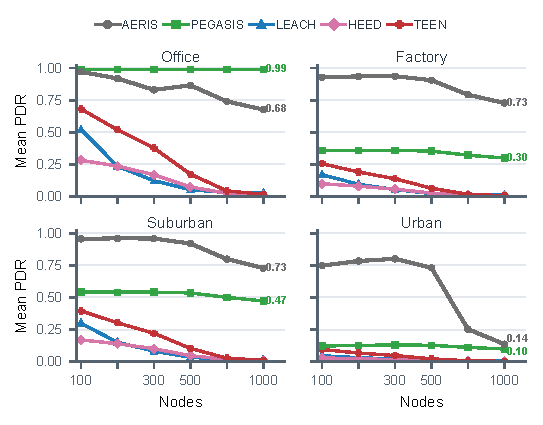
\includegraphics[width=\columnwidth]{fig_lcn26_strict_compact.pdf}
\caption{\textbf{Stress layer.}\, Collision-aware adapted Python stress test across four environments and 100--1000 nodes ($n=3200$ per cell). LEACH, HEED, and TEEN are minimally relay-enabled; this layer tests collision-and-relay stress and is not canonical ranking evidence.}
\label{fig:strict_python}
\end{figure}

\subsection{Ablation and Deployment Boundary}
Figure~\ref{fig:ablation} gives the expanded NS-3 module attribution test. It compares full AERIS with three ablated variants over the four-environment, seven-scale matrix used in the boundary sweep, for 3360 experiments in total. The result is sharper than the earlier fixed 100-node ablation: Gateway is the main gain carrier in factory and suburban cells. Removing Gateway costs 5.82 percentage points on average in factory and 7.58 points in suburban, with all seven node scales significant after Holm correction in both environments. It is essentially neutral in office and weak in urban, which matches the boundary result: office does not need extra uplink protection, while urban links can become too poor for a nearby Gateway to rescue reliably.

\begin{figure}[t]
\centering

\includegraphics[width=\columnwidth]{fig_lcn26_ns3_ablation_expanded.pdf}
\caption{Expanded NS-3 AERIS ablation summary across four environments and 50--1000 nodes ($n=30$ per cell). Horizontal bars show mean PDR contribution of each module across the seven node scales; whiskers give the per-environment min/max range. Positive values indicate that the module improves PDR; negative values indicate that removing the module improves PDR. Labels append $(k/7)$, the number of node scales with significant full-minus-ablated differences after Welch tests with Holm correction.}
\label{fig:ablation}
\end{figure}

CAS behaves differently. Removing CAS is beneficial in office and suburban cells, but hurts urban delivery by 0.91 points on average, with five of seven urban scales significant. CAS is therefore not a universal gain module; it is useful mainly when a short local detour remains viable under harsh links. Removing the CH scoring component is near-neutral in all environments. That does not make the score irrelevant to the design, but it does show that the measured delivery gain in this publication configuration should not be attributed to head scoring.

\subsection{Mechanism and Deployment Trade-off}
The 400-replicate-per-cell mechanism matrix is summarized in Fig.~\ref{fig:mechanism}. Gateway uplink PDR stays near 1.0 in office, factory, and suburban cells, but drops sharply at urban-1000, exactly where end-to-end PDR collapses. A targeted replication of the three harsh 1000-node cells on an independent machine reproduced the same bottleneck pattern to the reported precision. The visual takeaway matches the ablation: Gateway carries the gain, CAS is conditional, and Skeleton remains dormant because Gateway support resolves most eligible fallback cases in this configuration. These cell-level FND values expose harsh-regime role exhaustion and are not directly comparable to the pooled 100-node block in Table~\ref{tbl:pooled_summary}.

\begin{figure}[t]
\centering

\includegraphics[width=\columnwidth]{fig_lcn26_mechanism_compact.pdf}
\caption{AERIS mechanism matrix from 400 replicates per environment-node cell across 12 cells (4800 runs total). Panels report end-to-end PDR, Gateway-uplink PDR, first-node death (FND), and CAS two-hop share without shared secondary axes. Early FND exposes the reliability-lifetime cost of concentrated relay roles.}
\label{fig:mechanism}
\end{figure}

\begin{table}[t]
\caption{Fixed 100-node block. Bold = proposed. AERIS has the highest pooled PDR; its lowest consumed energy reflects forwarding-role exhaustion (shortest lifetime, earliest FND), not isolated efficiency. FND right-censored at 300 rounds; NR = no first-node death observed before horizon.}
\label{tbl:pooled_summary}
\centering
\scriptsize
\setlength{\tabcolsep}{2pt}
\begin{tabular*}{\columnwidth}{@{\extracolsep{\fill}}lccccc@{}}
\toprule
Method & PDR$\uparrow$ & Consumed J$\downarrow$ & Lifetime$\uparrow$ & FND$\uparrow$ & Hops$\downarrow$ \\
\midrule
LEACH & 0.260 & 165.4 & 300.0 & NR & 1.71 \\
HEED & 0.414 & 165.2 & 300.0 & 11.4 & 2.00 \\
TEEN & 0.432 & 159.4 & 299.0 & NR & 1.28 \\
PEGASIS & 0.373 & 137.6 & 300.0 & 70.7 & 32.37 \\
\midrule
\textbf{AERIS} & \textbf{0.674} & \textbf{131.1} & \textbf{215.5} & \textbf{15.8} & \textbf{1.98} \\
\bottomrule
\end{tabular*}
\end{table}

The cost is just as clear. Table~\ref{tbl:pooled_summary} shows that AERIS records the lowest consumed energy (131.1 J), but this value reflects early forwarding-role exhaustion rather than an isolated efficiency advantage; it also has the shortest lifetime (215.5 rounds), confirming that delivery is bought with concentrated relay burden. Fig.~\ref{fig:mechanism} localizes the cost to early node death and shrinking two-hop support in harsh cells.

Figures~\ref{fig:ns3_boundary}--\ref{fig:ablation} and Table~\ref{tbl:pooled_summary} suggest a concrete deployment rule. Prefer PEGASIS-like routing when lifetime dominates in benign cells; consider mature CTP/RPL-style stacks first when richer collection-tree control is acceptable, especially in office, factory, or urban regimes; choose AERIS when delivery under heterogeneous harsh links is the priority and a simple auditable controller is required, especially in suburban-like cells. Office-like regimes, longevity-first deployments, and mature LLN stacks are the clearest negative cases.

\section{LIMITATIONS}
Several concrete limits remain. The boundary sweep includes only simplified CTP- and RPL-MRHOF-style collection baselines, not opportunistic routing, ORW/ORPL-style candidate forwarding, coding-based reliability, channel hopping, or standards-compliant Contiki-NG/TinyOS RPL stacks; the AERIS--baseline ordering should therefore be read as a controlled collection-style comparison rather than a direct claim against full LLN stacks. The collision-aware stress layer is deployment-stress evidence rather than real-radio-testbed ground truth, and its MAC abstraction omits full 802.15.4/TSCH/CSMA-CA behavior.

Because TEEN is event-triggered, $\mathrm{PDR}_{\mathrm{expected}}$ should be read together with energy, lifetime, FND, and hops; actual-transmission PDR or event-detection success would be needed for a TEEN-centered study. Topology is static, and the environment taxonomy is bounded to the four tested regimes. Recent LLN work likewise emphasizes scalable path management and control-plane flexibility \cite{almutairi2024survey,djennadi2025exploring}. The provenance chain separates native-harness evidence from stress evidence, and a targeted replication of the three harsh 1000-node mechanism cells reproduced the key bottleneck means. All AERIS coefficients and thresholds are fixed once before evaluation; the implementation and raw results will be released publicly upon acceptance.

\section{CONCLUSION}
This paper presented and evaluated AERIS through a five-protocol NS-3 comparison, a seven-protocol boundary sweep, a collision-aware stress layer, and a mechanism study. The claim is deliberately bounded: AERIS is a reliability-first alternative to classical WSN baselines, but richer collection-tree routing narrows or removes that advantage in office, factory, and urban regimes. The practical contribution is a visible deployment boundary rather than a universal ranking. Future work should compare against full RPL/ORW/ORPL-style stacks and more realistic MAC behavior, then test whether Gateway-style reinforcement can coexist with collection-tree parent selection without reproducing the early-node-death cost.

\FloatBarrier
\bibliographystyle{IEEEtran}
\bibliography{ref}

\end{document}
